\documentclass[a4paper]{article}%

\usepackage[english]{babel}%
\usepackage[utf8]{inputenc}%
\usepackage[T1]{fontenc} %

\usepackage{graphicx}%
\usepackage{xspace}%

\usepackage{amsmath}
\usepackage{amsfonts}
\usepackage{amssymb}

\usepackage[margin=2.5cm]{geometry}

\usepackage{caption}
\usepackage{subcaption}
\usepackage{float}  % H option for figures

\DeclareMathOperator{\E}{E}
\DeclareMathOperator{\Cod}{Cod}
\newcommand{\CodSk}{\overset{\sim}{\Cod}}


\begin{document}

\title{Project IRESI}

\author{Simon Bihel, Florestan De Moor \\ ENS Rennes, Computer Science Department, 1st year}

\date{November 22, 2015}

\maketitle

\begin{abstract}
	In this report we present our work on the project of the course IRESI. We will first explain how we implemented the \texttt{SketchMin} algorithm, which is a metric used to detect DDoS. We coded this using the Python 3 language. We will then compare the results of the algorithm to exact values.
\end{abstract}


\section{DDoS and server security}

A DDoS (Distributed Denial of Service) attack is nowadays a well-known issue : it consists of sending a huge number of requests to a server, so that it crashes, and therefore to make it unavailable for the other users. The requests are sent to the server by the router, which receives data streams. If the attack is concentrated in a single stream, it is easy do detect it. However, if the attack is scattered among several streams, it is much more difficult to detect it.

\paragraph{}That's why the following method was implemented : the router receives different data streams, and calculates for each peer a correlation indicator which is the codeviance of the frequency vectors corresponding to the streams. The codeviance formulas are presented below in section \textbf{2.2}. Once this was computed, it becomes possible to determine if an attack is happening or not, by analyzing the codeviance values.

\paragraph{}Nevertheless, the stream sizes are huge, we can't afford to calculate the precise codeviance. The \texttt{SketchMin} algorithm is an easier way to calculate an estimated codeviance using hash functions in which precision is controlled by a set of parameters ($\varepsilon, \delta)$. We will present in next section how we implemented it using the Python 3 language. We will then compare its results with exact values in section \textbf{3}, by running it with real and randomly generated data traces.


\section{Programming the SketchMin algorithm}
% mini intro 2l
For the detection we need to first select the entries to then apply the algorithm that will produce the material in which we will find whether or not there is an attack.

\subsection{Extracting information from data traces}
% Simon
%Translate if needed to integers. Extract all at once to find correlation ??? Could be repetitive with subsection Real data traces.

In data traces, each line correspond to a request made to the server. To extract a certain kind information, like the source of a request, there is just to go through each line which represent a line. And each time split the line based on white-spaces and extract a certain entry. The entries are put in a list, and if needed are converted to integers without losing the fact that some entries are identical and others different. This can be done by creating a list of the distinct elements and the converting each element of the original list to the its index in the distinct elements list.

\paragraph{}This process has to be extended to the extraction of multiple traces in a single time because what we want in the end is eventually find correlation between multiple traces. To do that the distinct elements list has just to be shared between the multiple extractions. And so, identical requests can be correlated after applying the \texttt{SketchMin} algorithm and act in reaction.

\subsection{Computing the codeviance}
% Florestan
First, we implemented two functions to compute the average, and codeviance of an array. To do this, we browse the array, and use the following formulas :
	\[ \E(X) = \frac{1}{|X|} \sum\limits_{x_i \in X} x_i \]
	\[ \Cod(X,Y) = \E(XY) - \E(X)\E(Y) \]
	
\paragraph{}We have in entry a data trace $D$, and precision parameters $(\varepsilon, \delta)$. We start by defining the following constants :
	\[ k =\left\lceil \frac{1}{\varepsilon} \right\rceil \]
$k$ is the number of partitions we will create.
	\[ t = \left\lceil \log(\frac{1}{\delta}) \right\rceil \]
$t$ is the number of hashing functions we will consider.
	
\paragraph{}The data trace has integers values which stand between $0$ and $u$. We have to define $t$ universal hashing functions $h_i$ :
	\[ h_i(x) = ((a_ix+b_i) \mod u) \mod k \quad \forall i \in \lbrace 1 \ldots t \rbrace \]
where $a_i, b_i$ are randomly generated in $\lbrace 1 \dots t-1 \rbrace$ for $a_i$, and $\lbrace 0 \ldots t-1 \rbrace$ for $b_i$.

\paragraph{}We can then create the partitions, and we get a matrix $R_{0 \leq i \leq t-1, 1 \leq j \leq k}$ where 
 	\[ R_{i,j} = \# \lbrace x \in D : h_i(x) = j \rbrace \]
 	
\paragraph{}We can now create a function that receive two data traces. It calculates the $D$ matrix for both trace, and then computes the codeviance :
	\[ \CodSk(D_1, D_2) = \underset{0 \leq i \leq t-1}{\min} \Cod(R_1[i], R_2[i]) \]
where $R[i]$ is the line $i$ of the matrix.

\paragraph{}We can then create the full codeviance matrix $C_{1 \leq i,j \leq p}$ when we have $p$ data traces :
	\[ C_{i,j} = \CodSk(D_i, D_j) \quad \forall i,j \in \lbrace 1 \ldots p \rbrace \]
We can notice that the codeviance is symmetrical (i.e. $\Cod(X,Y) = \Cod(Y,X)$). That's why only $p(p+1)/2$ computations are made to create this matrix (instead of $p^2$).

\paragraph{}Once we calculated this matrix, we can plot it in 3D to have a visual result.



\section{Experimental results}
% mini intro 2l
To evaluate the correctness of the algorithm, we just need to see if the results have the same appearance than the real values, with possibly a larger scale.

\subsection{Real data traces}
% Simon
% Extracting all at once to maybe find correlation, even after applying the bijection. Extracting the file-names cause the third kind of traces was unusable if we wanted to analyze the sources, as it only says if an internal or external request.

For the real traces, we used the file-names as entries for the algorithm, after converting them to integer by simply matching the index of the distinct elements. We used file-names because the calgaryaccess traces didn't really have an entry for the sources of the requests, and we wanted a consistent information extraction over the multiple traces to eventually find correlations.

Here are the rest of the parameters for the experiment :
% Just giving the parameters and putting the screenshots

\begin{itemize}
	\item $\varepsilon = 0.001$
	\item $\delta = 0.001$
\end{itemize}

In the figure~\ref{ref:exp_real} we can see the result of the experiment where the result of the algorithm is close to the original.


\begin{figure}[H]
	\center
	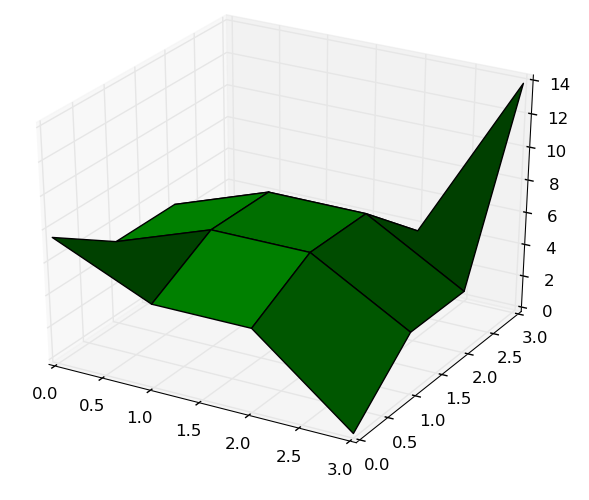
\includegraphics[scale=0.35]{realtests_real1.png}
	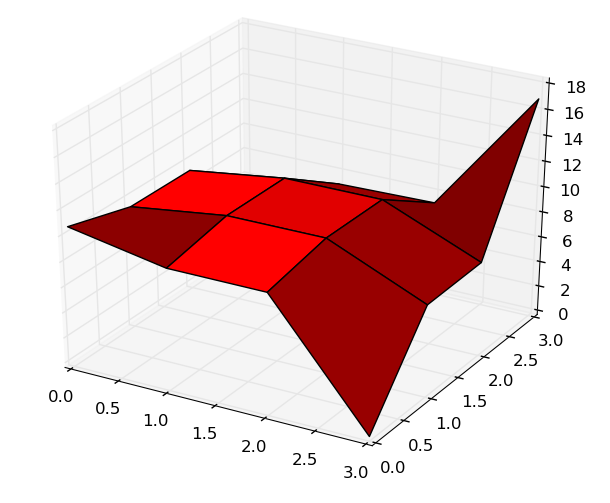
\includegraphics[scale=0.35]{realtests_sketchmin1.png}
	\caption{\footnotesize Codeviance matrix of real data traces: \\ real one (green) - calculated with \texttt{SketchMin} algorithm (red)}
	\label{ref:exp_real}
\end{figure}



\subsection{Generated data traces}
% Florestan

We generated artificial data traces using some probabilistic laws. Here are the parameters of this experiment :
\begin{itemize}
	\item size of the traces : $size = 10 000$
	\item integers values are generated between $0$ and $u = 100$
	\item $\varepsilon = 0.1$
	\item $\delta = 0.001$
\end{itemize}

\begin{center}
	\begin{tabular}{|c|c|c|}
		\hline
		 & Probabilistic laws & Parameters \\
		 \hline
		Trace 0 & Uniform & \\
		Trace 1 & Zipfian & $\alpha = 2$ \\
		Trace 2 & Zipfian & $\alpha = 3$ \\
		Trace 3 & Zipfian & $\alpha = 4$ \\
		Trace 4 & Zipfian & $\alpha = 5$ \\ 
		Trace 5 & Zipfian & $\alpha = 6$ \\
		Trace 6 & Poisson & $\lambda = u/(2)$ \\
		Trace 7 & Poisson & $\lambda = u/(2^2)$ \\
		Trace 8 & Poisson & $\lambda = u/(2^3)$ \\
		Trace 9 & Poisson & $\lambda = u/(2^4)$ \\
		Trace 10 & Poisson & $\lambda = u/(2^5)$ \\
		Trace 11 & Binomial & $p = 0.42$ \\
		Trace 12 & Negative Binomial & $p = 0.42$ \\
		\hline
	\end{tabular}
\end{center}


We calculated the real codeviance matrix, and we applied the \texttt{SketchMin} algorithm. Here are the results we got in figure~\ref{ref:exp_artificial} below. We can notice that the two shapes are really similar.

\begin{figure}[H]
	\centering
	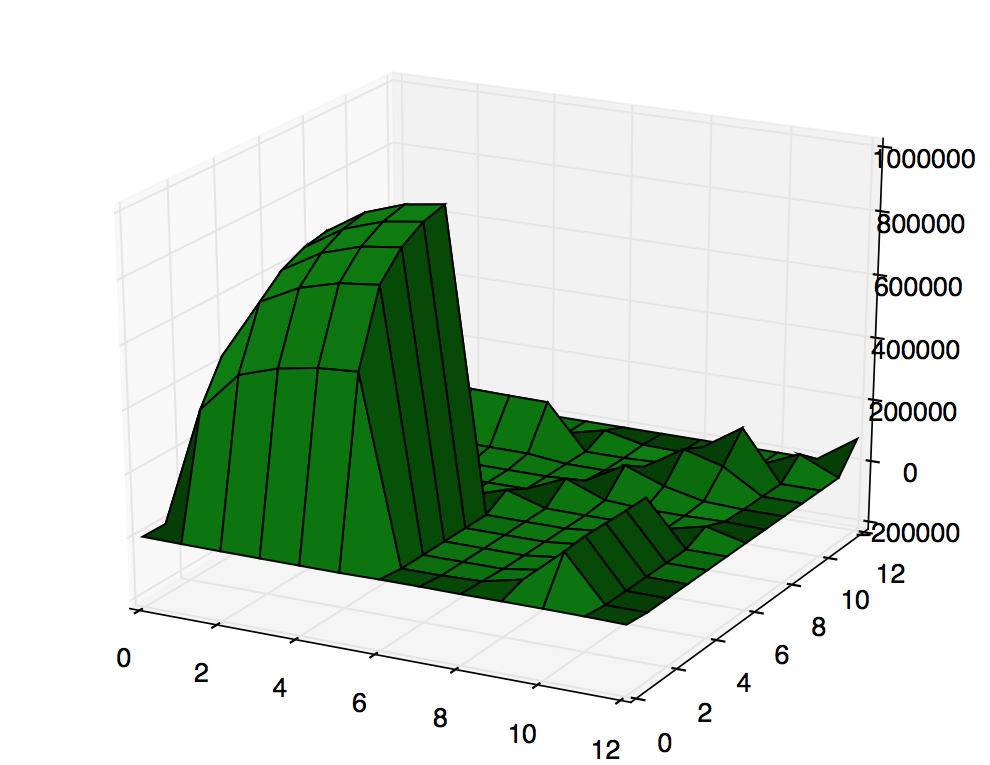
\includegraphics[scale=0.23]{generated_real.png}
	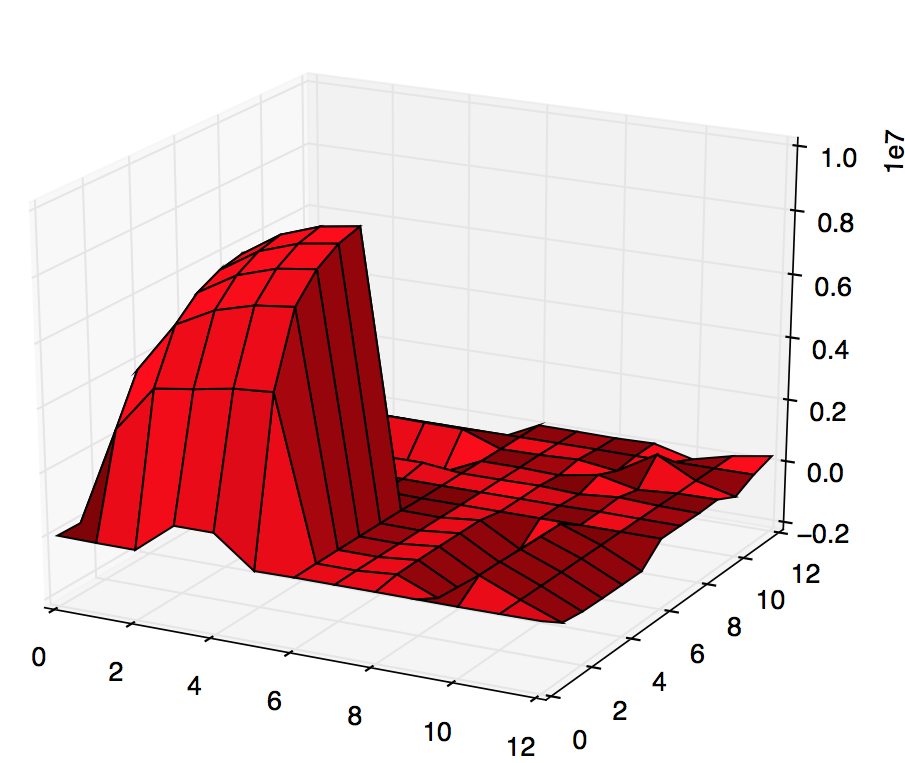
\includegraphics[scale=0.23]{generated_sk.png}
	\caption{\footnotesize Codeviance matrix of generated data traces:\\real one (green) - calculated with \texttt{SketchMin} algorithm (red)}
	\label{ref:exp_artificial}
\end{figure}


\section*{Conclusion}
% Simon / Florestan
% results look like exact entries
% what next ? -> find the right parameter to detect a false (=vicious) pike of activity
% what next ? -> put in concurrency the seperate codeviance computings

\clearpage

\end{document}